\documentclass[journal]{IEEEtran}
\usepackage[utf8]{inputenc}
\usepackage[portuguese]{babel}
\usepackage{lipsum}
\usepackage{cite}
\usepackage{graphicx}
\usepackage{tabularx}
\usepackage{algorithm}
\usepackage{algpseudocode}
\usepackage{hyperref}
\usepackage{amsmath}
\usepackage{amssymb}
\usepackage{subcaption}
\usepackage{float}
\usepackage{booktabs}

\newcommand{\figref}[1]{(\textbf{Fig.~\ref{#1}})}
\newcommand{\tabref}[1]{(Tab.~\ref{#1})}

\begin{document}
    \title{Influências Climáticas na Diminuição da Velocidade da Corrente do Golfo}
    \author{Duarte, T. S.}

    \maketitle

    \begin{abstract}
        Neste estudo, explora-se a Corrente do Golfo por meio de dados oceanográficos de temperatura superficial. Foi analisado o impacto do aquecimento global e do derretimento do gelo polar na velocidade da corrente e sua relação com o clima europeu. A análise, abrangendo o período de 1800 a 2022, incorporou 4.287.465 medições oceanográficas obtidas em 336.286 cruzeiros ou estações. Foram realizadas análises de distribuições temporais e geoespaciais, além de correlação e causalidade, revelando a ausência de conexões causais substanciais entre a temperatura superficial da Europa e a temperatura e salinidade da Corrente do Golfo. Ademais, investigou-se a hipótese de invernos cada vez mais rigorosos na Europa, porém as evidências encontradas foram inconclusivas.
    \end{abstract}

    \section{Introdução}
        A Circulação Termohalina representa um sistema complexo, caracterizado pelo movimento contínuo de grandes massas de água oceânica em todos os oceanos do mundo. Dentro desse sistema, um segmento notável é a \textit{Corrente do Golfo}. Essa corrente desempenha um papel vital no equilíbrio climático e biológico do Atlântico Norte, transportando água quente das regiões equatoriais do Oceano Atlântico até a costa ocidental da Europa. Ao chegar, essa água se resfria e afunda, iniciando seu retorno ao Golfo do México \figref{fig:img_corrente_golfo}.
        \begin{figure}[ht]
            \centering
            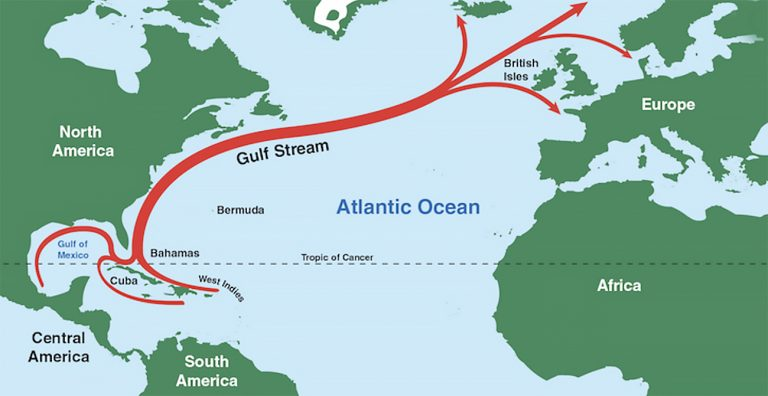
\includegraphics[width=0.95\linewidth]{/home/dusoudeth/Documentos/github/iof0201-gulf-stream/docs/artigo/img_corrente_golfo.jpg}
            \caption{Circulação Termohalina.}
            \label{fig:img_corrente_golfo}
        \end{figure}
        Esta dinâmica mantém o clima da Europa mais ameno do que o de outras regiões na mesma latitude, atuando como uma 'bomba de calor'. No entanto, estudos recentes indicam uma diminuição na velocidade média desta corrente, sendo que as variações de velocidade são altamente dependentes da região geoespacial \cite{Dong2019}, o que implica em mudanças climáticas significativas para a Europa, especialmente em períodos de inverno, que tendem a se tornar mais rigorosos. \newline
        Do ponto de vista hidrodinâmico, qualquer corpo de água possui uma densidade que é função da temperatura, composição química e pressão. Em corpos de águas marinhos, a densidade é fortemente influenciada pela salinidade. Assim, temos \(\rho = \rho(S, T, p)\), onde, a uma pressão constante, a densidade pode ser expressa por um par de equações.
        \begin{equation}
            \left\{\begin{matrix}
                \rho(S) = \rho_0 + \beta (S - S_0) \\
                \rho(T) = \rho_0 - \alpha (T - T_0)
            \end{matrix}\right.
        \end{equation}
        onde \(\rho_0\) representa a densidade da água do mar, \(\alpha\) e \(\beta\) são, respectivamente, os coeficientes de expansão térmica e salina, e \(S_0\) e \(T_0\) são os valores de referência para salinidade e temperatura. Com isso, são propostas as seguintes hipóteses:
        \begin{itemize}
            \item A uma pressão constante, o aumento da temperatura global e, consequentemente, a temperatura do oceano, reduz a densidade da água do mar.
            \item A uma pressão constante, o derretimento das calotas polares e, por conseguinte, a diluição do sal na água do mar, também reduz a densidade da água do mar.
        \end{itemize}
        Na literatura, estudos como \cite{Bromley2018,Cheng2019} apontam na direção da confirmação de ambas as hipóteses. Portanto, é razoável supor que o aumento da temperatura global e o derretimento das calotas polares estão diminuindo a densidade da água do mar, o que, por sua vez, reduz a velocidade da Corrente do Golfo. Este é um fenômeno em curso e que deve ser observável em dados reais.

    
    \section{Métodos}
        \subsection{Hardware e Software}
            Todas as análises foram realizadas em um sistema operacional \textit{Ubuntu Linux 22.04} de 64 bits, com 16 GB de RAM e um processador \textit{AMD Ryzen 7 3700X} de 8 núcleos. Utilizou-se uma unidade de processamento gráfico \textit{NVIDIA GeForce GTX 1660 Ti}. A implementação e execução dos códigos foram feitas em \textit{Python} versão 3.10.12. O código-fonte está disponível no repositório do GitHub \textit{iof0201-gulf-stream}\cite{iof0201_gulf_stream_2024}. As solicitações ao NOAA WOD retornam arquivos criptografados .OSD, os quais foram lidos utilizando a biblioteca python \textit{wodpy}.

        \subsection{Dados}
            Foram utilizadas duas principais fontes de informação para a análise: primeiramente, dados oceanográficos selecionados por meio do \textit{WODSelect} do projeto NOAA\cite{noaa_ncei_world_ocean_db_2024}, que fornece dados com base em critérios definidos pelos usuários \figref{fig:img_lat_lon_mar}. Os critérios aplicados neste trabalho foram:
            \begin{itemize}
                \item Latitude: $[10, 60]$
                \item Longitude: $[-80, 10]$
                \item Medidas: OSD
            \end{itemize}
            onde OSD representa \textit{Ocean Station Data}, isto é, dados coletados por estações fixas ou expedições, geralmente obtidos por navios, boias e plataformas de petróleo, em diferentes profundidades e para valores fixos de latitude e longitude. A segunda fonte de dados utilizada foi a de temperatura superficial da Europa, medida pelo projeto \textit{Berkeley Earth}\cite{berkeley_earth_surface_temp_2024}. Neste caso, o critério de seleção foi o nome do país. Os países escolhidos, banhados pelo Oceano Atlântico Norte, foram: Bélgica, Dinamarca, França, Irlanda, Itália, Países Baixos, Polônia, Portugal, Espanha e Reino Unido \figref{fig:img_lat_lon_europe}.
            \begin{figure}[ht]
                \centering
                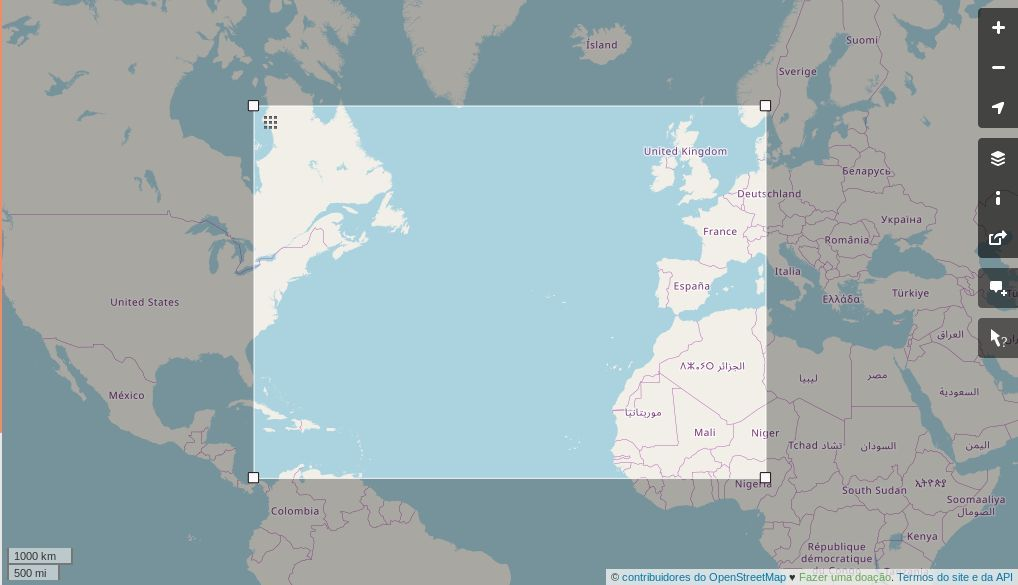
\includegraphics[width=0.95\linewidth]{/home/dusoudeth/Documentos/github/iof0201-gulf-stream/docs/artigo/img_lat_lon_mar.png}
                \caption{Recorte geoespacial dos dados oceanográficos, com a região de interesse destacada. A imagem foi obtida a partir do site OpenStreetMap.}
                \label{fig:img_lat_lon_mar}
            \end{figure}
            \begin{figure}[ht]
                \centering
                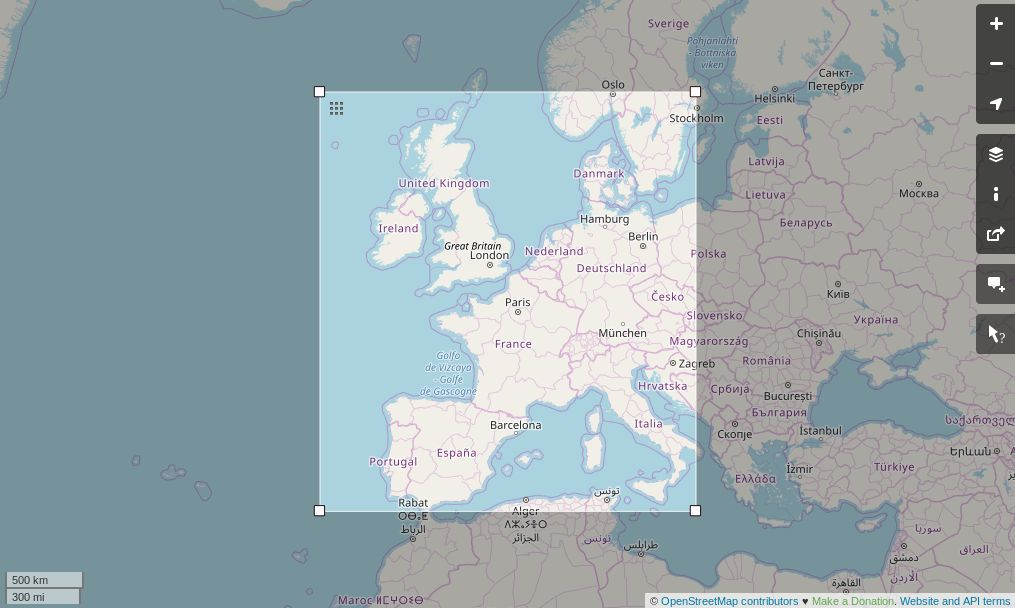
\includegraphics[width=0.95\linewidth]{/home/dusoudeth/Documentos/github/iof0201-gulf-stream/docs/artigo/img_lat_lon_europe.png}
                \caption{Recorte geoespacial dos dados de temperatura superficial da Europa, com a região de interesse destacada. A imagem foi obtida a partir do site OpenStreetMap.}
                \label{fig:img_lat_lon_europe}
            \end{figure}
    
    \section{Análise}
        \subsection{Análise Descritiva e Tratamento dos Dados Oceanográficos}
            Os dados oceanográficos analisados compreendem 4.287.465 medidas, obtidas em 336.286 cruzeiros ou estações, durante o período de 1800 a 2022. A distribuição geoespacial destas medidas é ilustrada na \figref{fig:img_hist_2d}. É notável que a maioria das medições ocorreu em latitudes próximas a 52 graus norte e longitudes em torno de -35 graus oeste. Para eliminar a influência da alta concentração de medidas na região mencionada, os pontos dessa área foram considerados outliers e excluídos da análise. Investigou-se também o impacto destes outliers em análises quantitativas. Verificou-se que, para as abordagens adotadas e descritas neste trabalho, a exclusão desses pontos não altera os resultados. Assim, a remoção serve principalmente para melhorar a clareza da análise qualitativa. O histograma ajustado, sem a inclusão desses outliers, é apresentado na \figref{fig:img_hist_2d_no_outliers}.
            \begin{figure}[ht]
                \centering
                \begin{subfigure}[b]{0.45\linewidth}
                    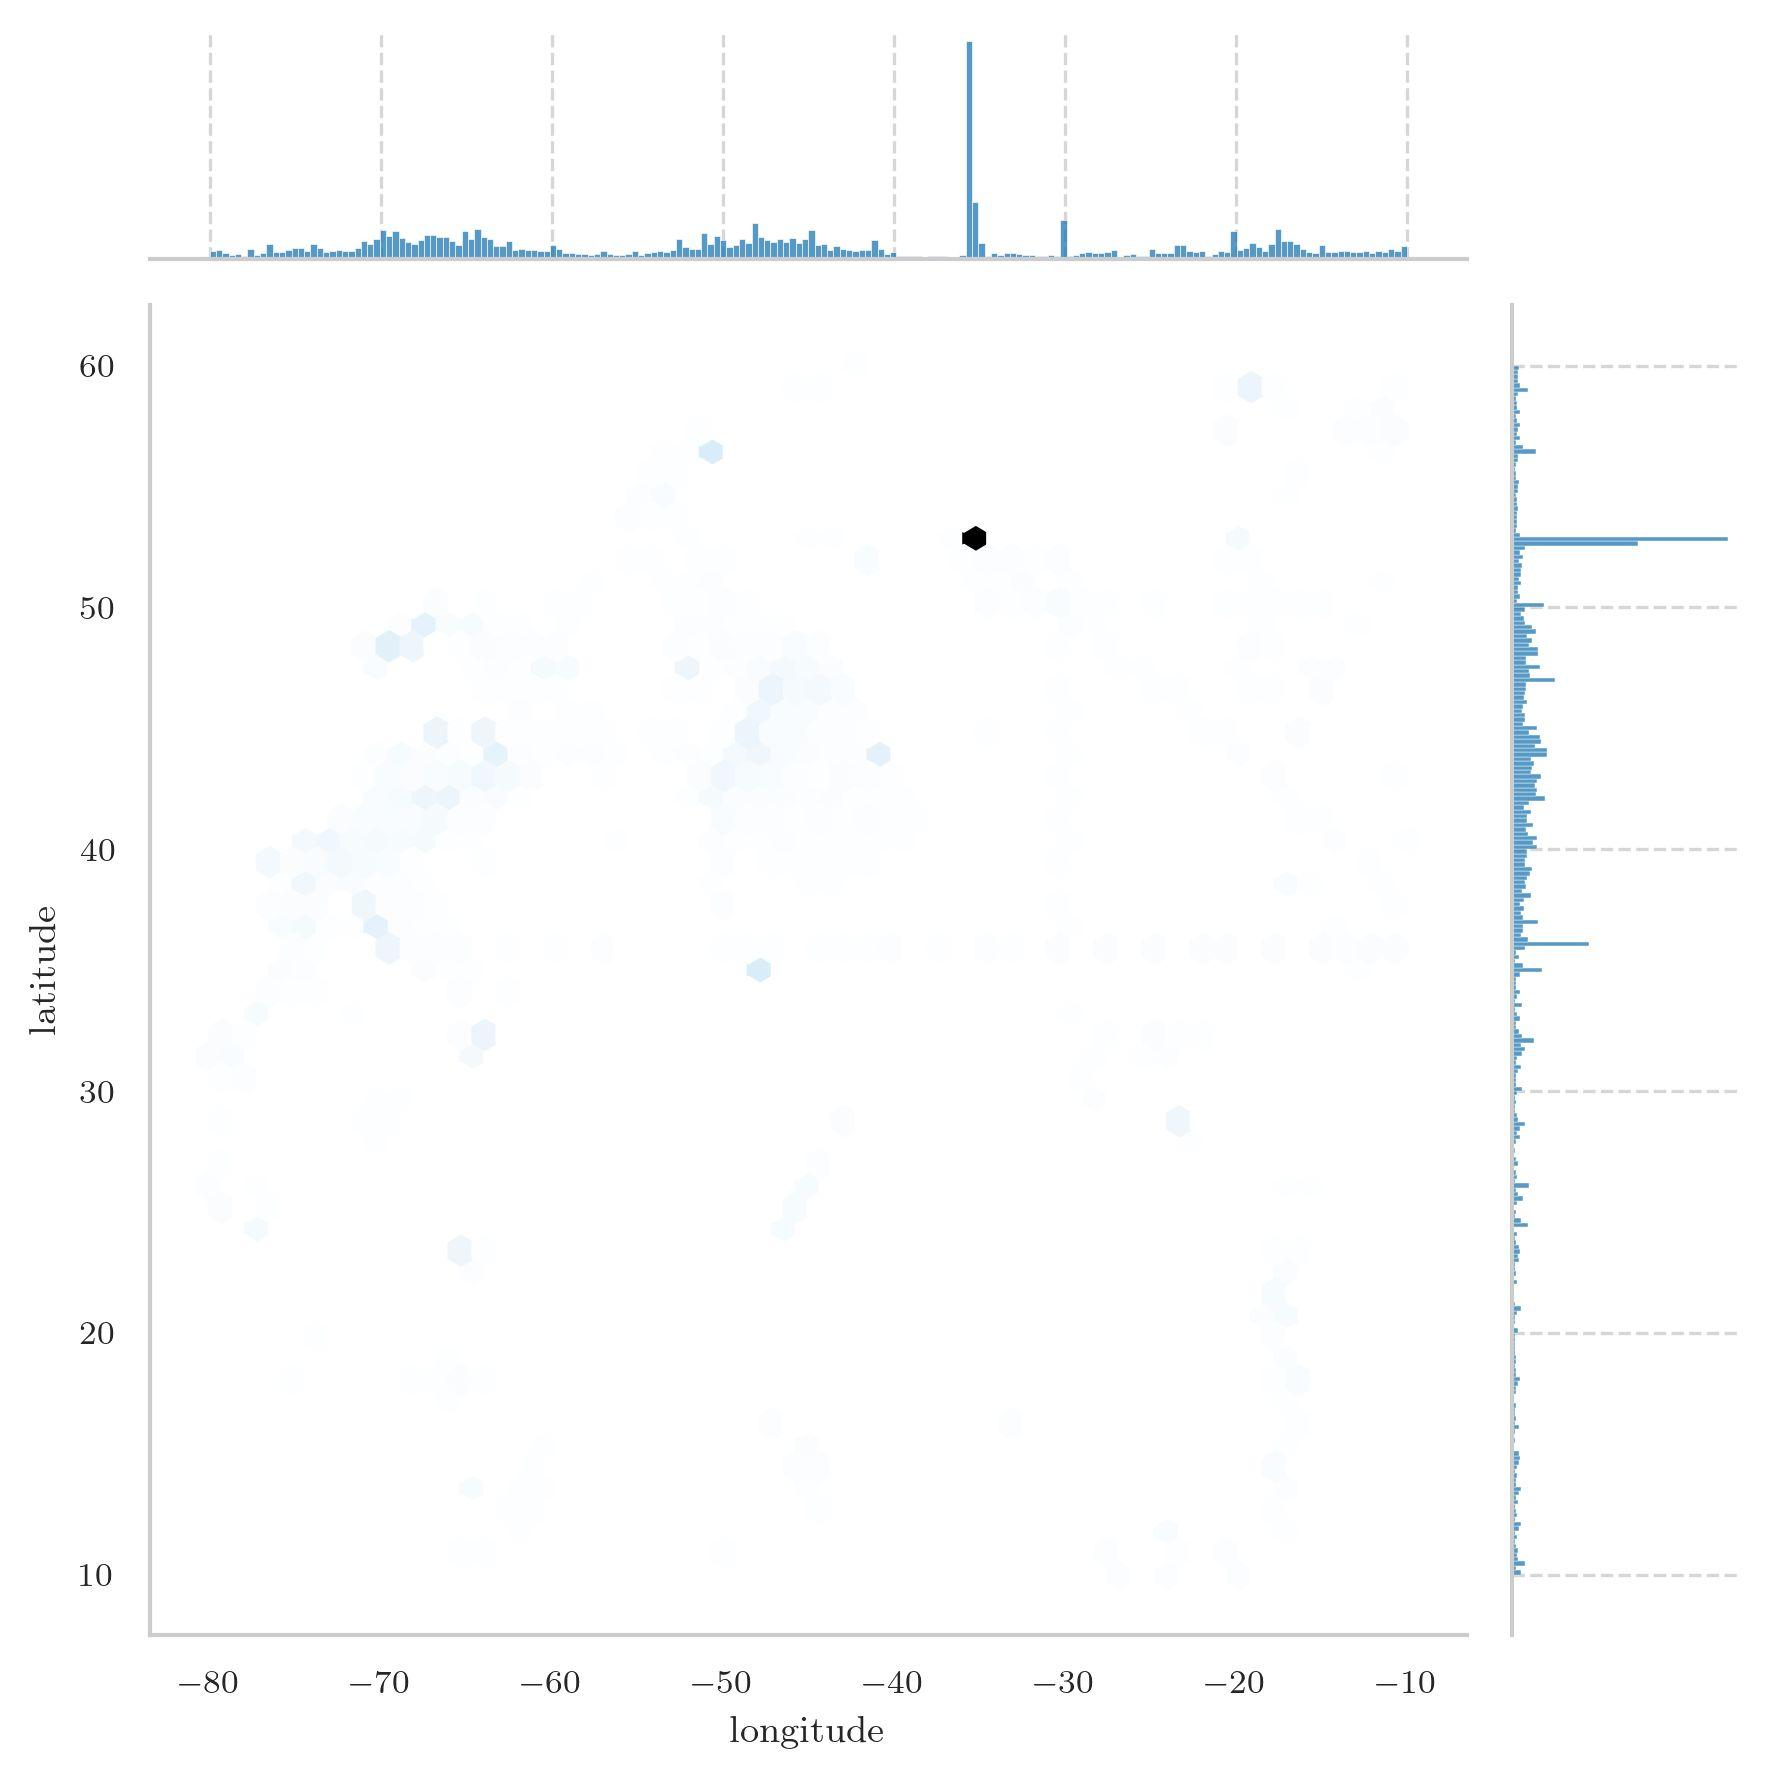
\includegraphics[width=\linewidth]{/home/dusoudeth/Documentos/github/iof0201-gulf-stream/docs/artigo/img_hist_2d.jpg}
                    \caption{Histograma 2D de pontos por latitude e longitude.}
                    \label{fig:img_hist_2d}
                \end{subfigure}
                \begin{subfigure}[b]{0.45\linewidth}
                    \includegraphics[width=\linewidth]{/home/dusoudeth/Documentos/github/iof0201-gulf-stream/data/08_reporting/points_distribution_no_outlier.png}
                    \caption{Histograma 2D de pontos sem outliers.}
                    \label{fig:img_hist_2d_no_outliers}
                \end{subfigure}
                \caption{Histogramas 2D de pontos por latitude e longitude com bins hexagonais.}
                % \label{fig:img_points_by_lon_lat_maps}
            \end{figure}

        \subsection{Análise Temporal e Geoespacial dos Dados Oceanográficos}
            A distribuição temporal das medidas é ilustrada na \figref{fig:img_number_of_points_per_year}, onde se observa um \emph{boom} de medições a partir de meados de 1950. Também é notável uma interrupção na coleta de dados por volta de 1917 e 1945, períodos que coincidem com a Primeira e a Segunda Guerra Mundial. Além disso, o terceiro gráfico desta figura mostra que, desde o início do registro de dados, houve medições em grandes profundidades, indicando que não existe uma tendência de intensificação na coleta de dados em profundidades cada vez maiores.
            \begin{figure}[ht]
                \centering
                \includegraphics[width=0.95\linewidth]{/home/dusoudeth/Documentos/github/iof0201-gulf-stream/data/08_reporting/number_of_points_per_year.png}
                \caption{Gráfico de distribuição temporal dos dados oceanográficos. O primeiro mostra o número de medidas por ano, o segundo o número de cruzeiros por ano e por profundidade, e o terceiro o número de medidas por profundidade.}
                \label{fig:img_number_of_points_per_year}
            \end{figure}
            Os histogramas de distribuição geoespacial dos dados oceanográficos, por latitude e longitude, sobrepostos com o contorno das costas dos continentes e ilhas revelam uma maior concentração de expedições no leste dos Estados Unidos \figref{fig:img_cruises_distribution_map}. Apesar disso, a maior concentração de medidas está localizada no meio do Oceano Atlântico Norte, entre a América do Norte e a Europa \figref{fig:img_points_distribution_map}.
            \begin{figure}[ht]
                \centering
                \begin{subfigure}[b]{0.45\linewidth}
                    \includegraphics[width=\linewidth]{/home/dusoudeth/Documentos/github/iof0201-gulf-stream/data/08_reporting/cruises_distribution_map.png}
                    \caption{Histograma 2D de cruzeiros por latitude e longitude.}
                    \label{fig:img_cruises_distribution_map}
                \end{subfigure}
                \begin{subfigure}[b]{0.45\linewidth}
                    \includegraphics[width=\linewidth]{/home/dusoudeth/Documentos/github/iof0201-gulf-stream/data/08_reporting/points_distribution_map.png}
                    \caption{Histograma 2D de medidas por latitude e longitude.}
                    \label{fig:img_points_distribution_map}
                \end{subfigure}
                \caption{Gráficos de cruzeiros e medidas por latitude e longitude.}
                % \label{fig:img_points_distribution_map}
            \end{figure}
            Ao analisar a distribuição de medidas por cruzeiro, nota-se que a maioria dos cruzeiros contém algumas dezenas de medidas \figref{fig:img_number_of_points_per_cruise}. 
            \begin{figure}[ht]
                \centering
                \includegraphics[width=0.95\linewidth]{/home/dusoudeth/Documentos/github/iof0201-gulf-stream/data/08_reporting/number_of_points_per_cruise.png}
                \caption{Gráfico de medidas por cruzeiro em escala logarítmica.}
                \label{fig:img_number_of_points_per_cruise}
            \end{figure}
            Além disso, a maior densidade de medidas está concentrada nos primeiros 1000 metros de profundidade \figref{fig:img_joyplot_points_by_depth_lon}\figref{fig:img_joyplot_points_by_depth_lat}.
            \begin{figure}[ht]
                \centering
                \includegraphics[width=0.95\linewidth]{/home/dusoudeth/Documentos/github/iof0201-gulf-stream/data/08_reporting/joyplot_points_by_depth_lon.png}
                \caption{Gráfico de distribuições de medidas por faixa de profundidade ao longo da longitude.}
                \label{fig:img_joyplot_points_by_depth_lon}
            \end{figure}
            \begin{figure}[ht]
                \centering
                \includegraphics[width=0.95\linewidth]{/home/dusoudeth/Documentos/github/iof0201-gulf-stream/data/08_reporting/joyplot_points_by_depth_lat.png}
                \caption{Gráfico de distribuições de medidas por faixa de profundidade ao longo da latitude.}
                \label{fig:img_joyplot_points_by_depth_lat}
            \end{figure}
            Por fim, as \figref{fig:img_points_distribution_by_month_1700_1950} e \figref{fig:img_points_distribution_by_month_1950_2023} mostram que as medidas oceânicas não representam toda a extensão da corrente do Golfo, e que as medidas estão satisfatoriamente bem distribuídas no tempo para captura de tendências temporais.
            \begin{figure}[ht]
                \centering
                \begin{subfigure}[b]{0.45\linewidth}
                    \includegraphics[width=\linewidth]{/home/dusoudeth/Documentos/github/iof0201-gulf-stream/data/08_reporting/points_distribution_by_month_1700_1950.png}
                    \caption{Gráficos de distribuição mensal de medidas ao longo dos anos 1700 a 1950.}
                    \label{fig:img_points_distribution_by_month_1700_1950}
                \end{subfigure}
                \begin{subfigure}[b]{0.45\linewidth}
                    \includegraphics[width=\linewidth]{/home/dusoudeth/Documentos/github/iof0201-gulf-stream/data/08_reporting/points_distribution_by_month_1950_2023.png}
                    \caption{Gráficos de distribuição mensal de medidas ao longo dos anos 1950 a 2023.}
                    \label{fig:img_points_distribution_by_month_1950_2023}
                \end{subfigure}
                \caption{Gráficos de distribuição mensal de medidas ao longo dos anos. Ambos os gráficos foram gerados de forma independente, de tal modo que o código de cores deve ser interpretado individualmente, com tons mais claros e amarelados indicando medidas mais antigas e tons mais escuros e avermelhados indicando medidas mais recentes.}
                % \label{fig:img_points_by_lon_lat_maps}
            \end{figure}
            Das análise descritivas e exploratórias realizadas, conclui-se que os dados oceanográficos não estão distribuídos de forma minimamente uniforme no espaço. No entanto, a distribuição temporal é satisfatória para a captura de tendências temporais. Ainda que técnicas de interpolação, regressão ou estratégias de agregação possam ser utilizadas para preencher as lacunas geoespaciais, optou-se por não fazê-lo, uma vez que a distribuição temporal é satisfatória para a análise proposta neste trabalho.

        \subsection{Comparação entre Dados Oceanográficos e Dados de Temperatura Superficial da Europa}
            Ao comparar as evoluções temporais da temperatura superficial da Europa, da temperatura do mar na região da Corrente do Golfo e da salinidade do mar na região da Corrente do Golfo, observa-se que a temperatura superficial da Europa apresenta uma tendência de aumento, enquanto a temperatura do mar na região da Corrente do Golfo apresenta uma tendência de diminuição \figref{fig:img_temperature_europe_gulf}. A salinidade do mar na região da Corrente do Golfo, por sua vez, apresenta uma tendência de aumento. 
            \begin{figure}[ht]
                \centering
                \includegraphics[width=0.95\linewidth]{/home/dusoudeth/Documentos/github/iof0201-gulf-stream/data/08_reporting/temperature_europe_gulf.png}
                \caption{Gráficos de evolução anual da temperatura superficial da Europa, da temperatura do mar na região da Corrente do Golfo e da salinidade do mar na região da Corrente do Golfo.}
                \label{fig:img_temperature_europe_gulf}
            \end{figure}
            Investigando cada série temporal individualmente, observa-se que a temperatura superficial da Europa apresenta uma tendência de aumento de 0.011 graus Celsius por ano \figref{fig:img_temperature_europe_gulf_lmplot}, a salinidade do mar na região da Corrente do Golfo apresenta uma tendência de aumento de 0.028 por ano \figref{fig:img_temperature_europe_gulf_lmplot_s} e a temperatura do mar na região da mesma região apresenta uma tendência de diminuição de 0.008 graus Celsius por ano \figref{fig:img_temperature_europe_gulf_lmplot_t}. 
            \begin{figure*}
                \centering
                \begin{subfigure}[b]{0.3\linewidth}
                    \includegraphics[width=\linewidth]{/home/dusoudeth/Documentos/github/iof0201-gulf-stream/data/08_reporting/temperature_europe_gulf_lmplot.png}
                    \caption{Evolução anual da temperatura superficial da Europa.}
                    \label{fig:img_temperature_europe_gulf_lmplot}
                \end{subfigure}
                \begin{subfigure}[b]{0.3\linewidth}
                    \includegraphics[width=\linewidth]{/home/dusoudeth/Documentos/github/iof0201-gulf-stream/data/08_reporting/temperature_europe_gulf_lmplot_t.png}
                    \caption{Evolução anual da temperatura do mar na região da Corrente do Golfo.}
                    \label{fig:img_temperature_europe_gulf_lmplot_t}
                \end{subfigure}
                \begin{subfigure}[b]{0.3\linewidth}
                    \includegraphics[width=\linewidth]{/home/dusoudeth/Documentos/github/iof0201-gulf-stream/data/08_reporting/temperature_europe_gulf_lmplot_s.png}
                    \caption{Evolução anual da salinidade do mar na região da Corrente do Golfo.}
                    \label{fig:img_temperature_europe_gulf_lmplot_s}
                \end{subfigure}
                \caption{Gráficos de evolução anual da temperatura superficial da Europa, da temperatura do mar na região da Corrente do Golfo e da salinidade do mar na região da Corrente do Golfo, com intervalos de confiança de 95\% preenchidos em azul, retas de regressão linear e valor de coeficiente angular da reta.}
                \label{fig:img_temperature_europe_gulf_lmplot_s_t}
            \end{figure*}\newline
            Essa análise mostra que esse conjunto de dados, combinados, não convergem para as mesmas conclusões dos resultados de \cite{Bromley2018,Cheng2019}.
            \begin{table}[ht]
                \centering
                \caption{Predictive Power Score Analysis}
                \begin{tabular}{|l|l|l|l|}
                \hline
                Variable X & Variable Y & PPScore & Model \\ \hline
                AverageTemperature & t & 0 & DecisionTreeRegressor \\ \hline
                AverageTemperature & s & 0 & DecisionTreeRegressor \\ \hline
                \end{tabular}
                \caption*{O PPScore é uma métrica que mede a capacidade de uma variável prever outra. O valor 0 indica que a variável X não é capaz de prever a variável Y.}
                \label{tab:pps}
            \end{table}
            \begin{table}[ht]
                \centering
                \caption{Mutual Information Score}
                \begin{tabular}{|l|l|}
                \hline
                Variables & Mutual Information Score \\ \hline
                (AverageTemperature, t) & 4.8675 \\ \hline
                (AverageTemperature, s) & 4.7095 \\ \hline
                \end{tabular}
                \caption*{O MIScore é uma métrica que mede o quanto saber a distribuição de uma variável ajuda a prever a distribuição de outra, sendo que o valor 0 indica que as variáveis são oriundas de distribuições independentes.}
                \label{tab:mi}
            \end{table}
            \begin{table}[ht]
                \centering
                \caption{Correlation Analysis}
                \begin{tabular}{|l|l|l|}
                \hline
                Method & Variables & Correlation \\ \hline
                Pearson & (AverageTemperature, t) & 0.0603 \\ \hline
                Pearson & (AverageTemperature, s) & 0.0658 \\ \hline
                Spearman & (AverageTemperature, t) & -0.1577 \\ \hline
                Spearman & (AverageTemperature, s) & 0.1189 \\ \hline
                \end{tabular}
                \caption*{O coeficiente de correlação de Pearson mede a correlação linear entre duas variáveis, enquanto o coeficiente de correlação de Spearman mede a correlação monotônica entre duas variáveis, sendo que o valor 0 indica que as variáveis não são correlacionadas.}
                \label{tab:correlation}
            \end{table}
            Apesar disso, é possível observar visualmente que os gráficos de \figref{fig:img_temperature_europe_gulf_lmplot_s_t} apresentam ruído suficiente para que análises baseadas em regressão linear não sejam confiáveis. Por conta disso foram realizadas análises de correlação, utilizando o coeficiente de correlação de Pearson e o coeficiente de correlação de Spearman, além de análises de causalidade, utilizando o \textit{Predictive Power Score} e o \textit{Mutual Information Score}. Os resultados são apresentados nas \tabref{tab:pps}, \tabref{tab:mi} e \tabref{tab:correlation}. De forma geral os resultados confirmam o que pode ser intuido visualmente: não há possibilidade de estabelecer relações de causalidade e nem sequer de correlação entre os dados de temperatura superficial da Europa e os dados de temperatura e salinidade do mar na região da Corrente do Golfo.\newline 

            Por fim, é possível tentar verificar o efeito da tese investigada, isto é, se os invernos na Europa estão se tornando mais rigorosos. Embora no gráfico da \figref{fig:img_temperature_europe_boxplot} não seja possível observar tendências claras, em particular na parte inferior dos \emph{boxes}, que indicam valores extremos, na \figref{fig:img_temperature_europe_overlapped} nota-se que as curvas de distribuição mensais de temperaturas mais recentes possuem as extremidades -- correspondentes aos meses de inverno -- levemente divergentes visualmente das regiões intermediárias das curvas, indicando que meses de inverno de anos recentes estão sendo mais frios.
            \begin{figure}[ht]
                \centering
                \includegraphics[width=0.95\linewidth]{/home/dusoudeth/Documentos/github/iof0201-gulf-stream/data/08_reporting/temperature_europe_boxplot.png}
                \caption{Distribuição de temperatura superficial da Europa por ano, agregada por mês.}
                \label{fig:img_temperature_europe_boxplot}
            \end{figure}
            \begin{figure}[ht]
                \centering
                \includegraphics[width=0.95\linewidth]{/home/dusoudeth/Documentos/github/iof0201-gulf-stream/data/08_reporting/temperature_europe_overlapped.png}
                \caption{Distribuições mensais de temperatura superficial da Europa, sobrepostas, com código de cores indicando o ano, onde tons mais claros e amarelados indicam anos mais antigos e tons mais escuros e avermelhados indicam anos mais recentes.}
                \label{fig:img_temperature_europe_overlapped}
            \end{figure}
    
    \section{Conclusão}
        Este estudo examinou a relação entre a Circulação Termohalina, especialmente a Corrente do Golfo, e o clima da Europa. Após uma análise detalhada dos dados oceanográficos e de temperatura superficial, constatou-se uma ausência de correlações claras entre a temperatura e salinidade do mar na região da Corrente do Golfo e as temperaturas superficiais da Europa. Embora os padrões temporais e espaciais dos dados tenham sido adequados para a análise, os resultados não corroboraram totalmente as hipóteses iniciais nem os estudos anteriores. 
    

    \newpage

    \bibliographystyle{IEEEtran}
    \bibliography{artigo}

\end{document}
